% IN54 - Lab report
% Fall 2014
% Authors : Adrien Berthet and Camille Mougin

%-------------------------------------------------------------------------------
%	PACKAGES AND DOCUMENT CONFIGURATIONS
%-------------------------------------------------------------------------------

\documentclass[a4paper,11pt]{article}
\usepackage[margin=1.3in]{geometry}
\usepackage[utf8x]{inputenc}
\usepackage[T1]{fontenc}
\usepackage[french]{babel}
\usepackage{color,colortbl}
\usepackage{fancyhdr}
\usepackage{graphicx}
\usepackage{hyphenat}	% Caesura
\usepackage{hyperref}	% Simple Link
\usepackage[]{algorithm2e} % Algorithm
\usepackage{amsmath}
\usepackage{amssymb}
\usepackage{kpfonts}

\setlength\parindent{0pt} % Removes all indentation from paragraphs

% Line break after itemize
\let\EndItemize\enditemize
\def\enditemize{\EndItemize\bigskip}

%-------------------------------------------------------------------------------
%	DOCUMENT INFORMATION
%-------------------------------------------------------------------------------

\title{Reconnaissance de chiffres\\Compte-rendu de TP - IN54}
\author{Adrien \bsc{Berthet} et Camille \bsc{Mougin}}
\date{UTBM - \bsc{Automne} 2014}

\begin{document}

\maketitle

%-------------------------------------------------------------------------------
%	CONTENT
%-------------------------------------------------------------------------------

% INTRODUCTION
\section*{Introduction}
L'objectif de ce TP est de réaliser un système complet de reconnaissance de chiffres manuscrits. Chaque chiffre sera d'abord isolé du reste, pour ensuite être analysé et classé par deux systèmes de classifications différentes. Ces classifieurs permettront d'obtenir une probabilité quant à la nature exacte du chiffre, et ces probabilités seront donc assemblées pour obtenir un résultat final.\\
Pour obtenir une probabilité, le système effectuera d'abord une séquence d'apprentissage, qui lui permettra d'avoir une base de données de comparaison.

Le schéma suivant donne un déroulement simple des différentes étapes permettant d'atteindre le résultat final.

% LOCALISATION DES CHIFFRES MANUSCRITS
\section{Pré-traitements : localisation et extraction des chiffres manuscrits}

Dans l'exemple étudié, la façon la plus simple de localiser les chiffres consiste d'abord à rechercher, à partir de l'histogramme de projections horizontales de pixels noirs, les plages correspondant à un nombre de pixels noirs non nul. Le début et la fin de chaque plage détectée sur l'histogramme des projections horizontales définissent une ligne de chiffres dans l'image. En appliquant le même principe (mais à partir d'un histogramme de projections verticales) sur chaque ligne détectée, on peut alors déterminer l'emplacement de chaque chiffre de l'image.

\subsection{Recherche des lignes}
Le principe est très simple, puisqu'il suffit dans un premier temps de parcourir chaque ligne pour vérifier qu'elle contient un pixel noir ou non. Pour accélérer le processus et parcourir rapidement l'image, un histogramme du nombre de pixels noirs est récupéré. Ceci est possible facilement car l'image est déjà binaire. On peut alors remarquer de façon évidente les différentes lignes. Les valeurs de celles-ci (début et fin) sont alors sauvegardées pour être réutilisées lors de la recherche des colonnes.

\begin{figure}[hm]
	\begin{center}
		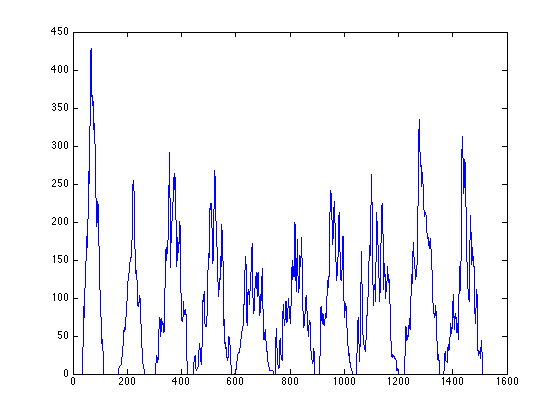
\includegraphics[width=0.8\textwidth]{img/10-black-level.png} 
	\end{center}
	\caption{Histogramme du niveau de noir}
\end{figure}
\newpage
\subsection{Recherche des colonnes pour chaque ligne}
Le même principe utilisé précédemment est recommencé, avec cette fois un histogramme du niveau de noir sur chaque colonne, pour une ligne unique (soit une ligne de chiffre). On obtient alors plusieurs histogrammes semblables au précédent, qui permettent d'obtenir un tableau avec les colonnes englobant chaque chiffre pour chaque ligne. 

\subsection{Détermination du rectangle englobant}
On pourrait penser qu'il n'y a plus d'étapes de découpe et qu'il faut uniquement assembler les coordonnées colonnes avec celles des lignes, mais il est nécessaire de repasser pour chaque chiffre dans le découpage des lignes, car ils possèdent un profil vertical beaucoup trop grand pour certains (puisqu'il s'agit du plus haut et plus bas chiffre pour chaque ligne). Ainsi, en effectuant une découpe plus précise, on obtient au final le résultat suivant.

\begin{figure}[hm]
	\begin{center}
		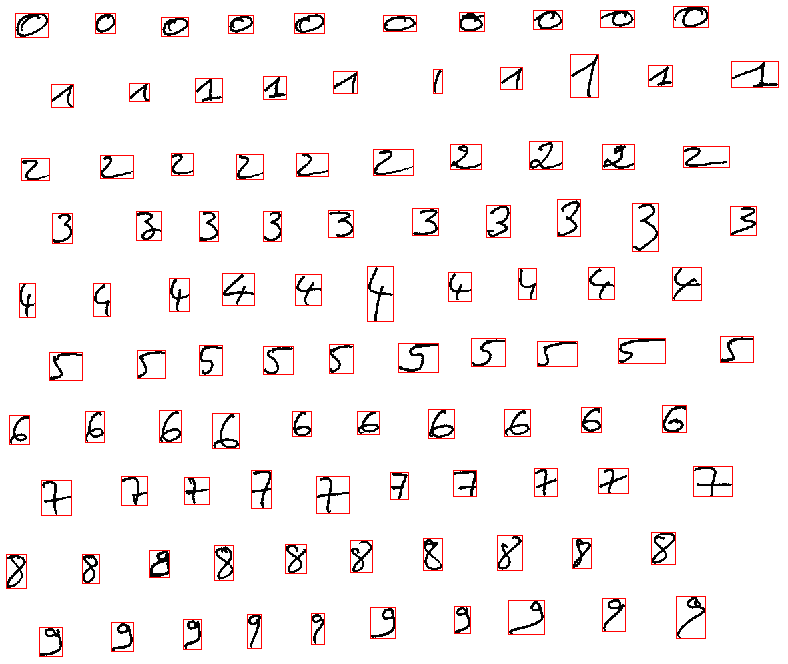
\includegraphics[width=0.8\textwidth]{img/11-final-cut.png} 
	\end{center}
	\caption{Résultat des découpes}
\end{figure}

\subsection{Avantages et inconvénients d'une telle méthode}
Cette méthode de localisation par projection est avantageuse puisque dans le cas ci présent, elle fournit un résultat parfait quant à la découpe des chiffres. Seulement, celle-ci peut perdre énormément en pertinence si les lignes de chiffres  n'étaient pas aussi droites.\\
Imaginons deux lignes consécutives, écrites de façon à ce qu'elles montent toutes les deux vers le haut. On se retrouve avec le premier chiffre de la première ligne qui se retrouve à la même hauteur que le dernier chiffre de la deuxième ligne. Ainsi, la méthode de l'histogramme ne convient pas du tout car on ne pourrait faire la différence entre les deux lignes.\\
On peut également remarquer que cette méthode devient vite lourde pour les images de grande taille et comprenant un nombre important de caractères (en plus de chiffres), et il serait donc pertinent de trouver une méthode plus optimisée.
\newpage

% CLASSIFIEUR 1 : PROFILS + DISTANCE EUCLIDIENNE MINIMUM
\section{Classifieur 1 : profils et classifieur par distance euclidienne minimum}

\subsection{Extraction des profils}
Chaque chiffre récupéré précédemment, il est désormais possible d'extraire les profils gauche et droit pour chacun, sur $d$ composantes. Ainsi, pour chaque chiffre, on utilise l'algorithme suivant :

\begin{figure}[h]
\begin{algorithm}[H]
	découper en 5 lignes avec $linspace$
	
	\For{chaque ligne}{
		\While{pixel\_gauche != noir}{
			profil gauche = pixel\_gauche + 1
		}	
		\While{pixel\_droit != noir}{
			profil droit = pixel\_droit - 1
		}
	}
	normaliser le profil obtenu
\end{algorithm}
\end{figure}

Enfin, on récupère tous ces profils et on les classe en fonction du chiffre auquel ils appartiennent, pour ensuite effectuer la moyenne des profils d'un même chiffre.

\subsection{Apprentissage du classifieur}

\subsection{Décision du classifieur}
\newpage

% CLASSIFIEUR 2 : DENSITES + KPPV
\section{Classifieur 2 : Densités et K plus proches voisins}
Liste des fonctions mentionnées dans ce chapitre : getdensity, computepdensities, learningclassifier2, decisionclassifier2

\subsection{Principe et implémentation}

Ce second classifieur vise à identifier un chiffre à partir des densités de pixels noirs obtenues dans les différentes zones qui le compose. La première étape consiste à diviser le rectangle encadrant le chiffre à identifier en m x n zones, puis de calculer la densité de pixels noirs dans chacune de ces zones.\\

Comme précédemment, le classifieur nécessite de passer par une phase d'apprentissage afin d'obtenir une base de densités de référence. Il est ensuite possible d'identifier le chiffre en comparant les densités obtenues avec les densités de référence. Les probabilités d'appartenance du chiffre à chacune des classes est finalement calculée en fonction du nombre de représentants de chaque classe parmis ses k plus proches voisins.

\subsubsection{Fonctions utilisées}

getdensity( rectangle, m, n ) : density
Entrées :
Calcule la densité de pixels noirs dans chaque zone de l'image. Les zones sont obtenues par division du rectangle contenant le chiffre en m parties sur la hauteur et n parties sur la largeur. Les densités sont calculées en divisant le nombre de pixels noirs décomptés par la hauteur x la largeur du rectangle.
Cette fonction retourne un vecteur de m x n composantes contenant les densités normalisées relatives à chaque zone.

computepdensities( vectordensity, vectordensitylearning, nbrectangleslearning, k ) : pbelonging
Entrées : 
Calcule la différence entre le vecteur de densités du chiffre à identifier et les vecteur de densités de chaque élément contenu dans la base d'apprentissage respectivement.



\subsubsection{Phase d'apprentissage}

learningclassifier2( rectangleslearning, learningimag, m, n) : vectordensitylearning


\subsubsection{Phase de décision}

decisionclassifier2( rectangles, image, vectordensitylearning, m, n, k) : pbelonging


\subsection{Analyse et conclusion}

\subsubsection{Résultats obtenus en fonction des paramètres m et n}

\subsubsection{Influence du paramètre k}
\newpage

% COMBINAISON DE CLASSIFIEURS
\section{Combinaison de classifieurs}

\subsection{Combinaison par somme et produit de probabilités}

Même si le second classifieur affiche un taux de reconnaissance plus élevé que le premier, on peut imaginer que les résultats obtenus puissent être complémentaires. C'est pourquoi, afin d'améliorer le taux de reconnaissance global du système, il est possible de combiner les probabilités obtenues par chaque classifieur afin d'obtenir un nouveau vecteur de probabilité d'appartenance. On espère le résultat ainsi obtenu plus précis que ceux donnés par leur utilisation indépendante,.\\
Deux méthodes de combinaison sont utilisées : la somme et le produit.\\
Soient pbelonging1 et pbelonging2 les probabilités d'appartenance respectivement obtenus pour les classifieurs 1 et 2. Les nouvelles probabilités, obtenues par combinaison en utilisant la somme et le produit, sont données de la façon suivante :

$$\begin{array}{rcl}
pbelongingsum(x/\omega_i) &=& pbelonging1(x/\omega_i) + pbelonging2(x/\omega_i)\\
pbelongingprod(x/\omega_i) &=& pbelonging1(x/\omega_i)pbelonging2(x/\omega_i)
\end{array}$$

avec $x$ l'objet testé pour la classe d'appartenance $\omega_i$


\subsection{Critique des résultats obtenus}

\begin{figure}[h]
	\begin{center}
		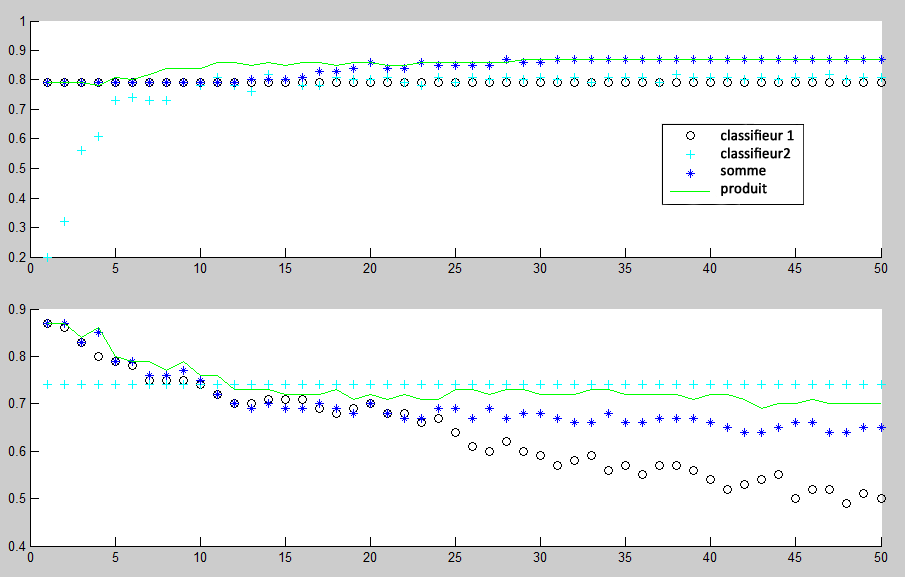
\includegraphics[width=\textwidth]{img/40-rates-function-of-d-k.png}
	\end{center}
	\caption{Variation des quatre taux de reconnaissance obtenus en fonction des paramètres $d$ (en haut) et $k$ (en bas)}
	\label{fig:ratecomparison}
\end{figure}

Globalement on observe de meilleurs résultats pour les combinaisons de classifieurs, représentés dans sur la figure ci-dessus en vert et en bleu foncé. Cependant, si l'on utilise les paramètres optimaux définis précédemment, les résultats sont biaisés : étant donné le paramètre $k$ fixé à 1, les probabilités résultant du second classifieur sont binaire, ce qui annule les résultats du premier classifieur dans le cas du produit mais aussi de la somme.

% CONCLUSION
\section*{Conclusion}

Les probabilités obtenues en fin de processus sont très correctes : 91\% de reconnaissance en optimisant les paramètres et combinant les classifieurs.\\
Cependant, de meilleurs résultats pourraient être obtenus en agrandissant la base d'apprentissage : en effet, nous avons vu que la méthode des k plus proches voisins n'est pas utilisée à hauteur de son potentiel étant donné que les meilleurs résultats sont obtenus en considérant seulement le voisin le plus proche. Les probabilités obtenues sont donc très contrastées ce qui limite l'action de la combinaison des classifieurs.\\
D'autre part, il semble que les chiffres de la base d'apprentissage ainsi que ceux à analyser aient été rédigés par une même personne, ce qui limite la différence de forme entre les chiffres. Pour obtenir des résultats significatifs, il faudrait idéalement varier les styles d'écriture dans la base d'apprentissage, ce qui réduirait le taux de reconnaissance mais améliorerait les performances réelles du système.

\end{document}
